\subsection{Regularyzacja}
Zajmijmy się regularyzacją naszego zbioru danych. Podzielmy zbiór na zmienne objaśniające (\textbf{X}) i zmienną objaśnianą (\textbf{y}).

\begin{Rcode}
X <- model.matrix(Installed_Capacity_MW ~ ., data = energy_data)[, -1]
y <- energy_data$Installed_Capacity_MW
\end{Rcode}

Wartość przyjmowane przez zmienne w zbiorze są bardzo duże, dlatego można spodziewać się wysokich wartości MSE.

\subsubsection{Regresja grzbietowa}
Rozpocznijmy regularyzację od przeprowadzenia regresji grzbietowej dla określonego ciągu \textbf{$\lambda$}

\begin{Rcode}
lambda_grid <- 10^seq(10, -2, length.out = 100)
fit_ridge <- glmnet(X, y, alpha = 0, lambda = lambda_grid)
\end{Rcode}

Zestaw estymat \textbf{fit\_ridge} to macierz o rozmiarch \textbf{13} (liczba kolumn) na \textbf{100} (długość lambda\_grid).

Sprawdźmy normy euklidesowe dla estymat:

\begin{Rcode}
fit_ridge$lambda[50]
coef_ridge <- coef(fit_ridge)[, 50]
coef_ridge
sqrt(sum(coef_ridge[-1]^2))
\end{Rcode}

Sprawdźmy to dla testowego MSE:

\begin{Rcode}
set.seed(1)
n <- nrow(X)
train <- sample(n, n / 2)
test <- -train
fit_ridge <- glmnet(X[train,], y[train], alpha = 0, lambda = lambda_grid,
                    thresh = 1e-12)
\end{Rcode}

Dla \(\boldsymbol{\lambda = 4}\):
\begin{Rcode}
pred_ridge <- predict(fit_ridge, s = 4, newx = X[test,])
mean((pred_ridge - y[test])^2)
\end{Rcode}

Otrzymujemy MSE na poziomie 83162.


Dla \(\boldsymbol{\lambda = 10^{10}}\):
\begin{Rcode}
pred_ridge_big <- predict(fit_ridge, s = 1e10, newx = X[test,])
mean((pred_ridge_big - y[test])^2)
\end{Rcode}

Otrzymujemy MSE na poziomie 83141.


Dla \(\boldsymbol{\lambda = 0}\), czyli po prostu dla \textbf{metody najmniejszych kwadratów}:
\begin{Rcode}
pred_ridge_0 <- predict(fit_ridge, x = X[train,], y = y[train], s = 0, 
                      newx = X[test,], exact = TRUE)
mean((pred_ridge_0 - y[test])^2)
\end{Rcode}

Otrzymujemy MSE na poziomie 83713.


Porównajmy estematy współczynników:
\begin{Rcode}
lm(y ~ X, subset = train)
predict(fit_ridge, x = X[train,], y = y[train], s = 0, exact = TRUE, 
        type = "coefficients")[1:13,]
\end{Rcode}

\begin{figure}[H]
    \centering
    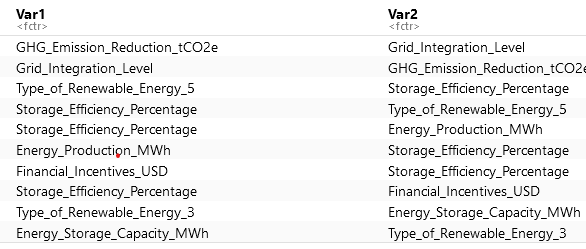
\includegraphics[width=1\linewidth]{lab4/obraz.png}
    \caption{Podusmowanie estymaty}
    \label{fig:enter-label}
\end{figure}

Wyliczmy optymalne estymaty przy pomocy walidacji krzyżowej:

\begin{Rcode}
set.seed(1)
cv_out <- cv.glmnet(X[train,], y[train], alpha = 0)
plot(cv_out)
cv_out$lambda.min
\end{Rcode}

\begin{figure}[H]
    \centering
    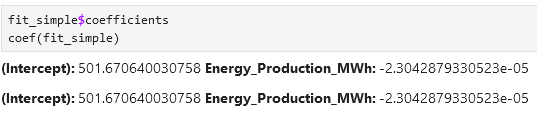
\includegraphics[width=1\linewidth]{lab4/obraz2.png}
    \caption{Zalezność między wartością MSE a $\lambda$}
    \label{fig:enter-label}
\end{figure}

Otrzymaliśmy optymalną wartość $\lambda \approx 8.3$. 

Estymaty współczynników dla optymalnej wartości $\lambda$:

\begin{figure}[H]
    \centering
    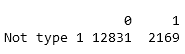
\includegraphics[width=1\linewidth]{lab4/obraz3.png}
    \caption{Intercept to estymata przy objaśnianiu zmiennej nią samą}
    \label{fig:enter-label}
\end{figure}

\subsubsection{Lasso}
Teraz spróbujemy wykorzystać metodę \textbf{L}east \textbf{A}bsolute \textbf{S}hrinkage and \textbf{S}election \textbf{O}perator - \textbf{LASSO}.

Dopasujmy LASSO do parametrów:

\begin{Rcode}
fit_lasso <- glmnet(X[train,], y[train], alpha = 1)
\end{Rcode}

\begin{figure}[H]
    \centering
    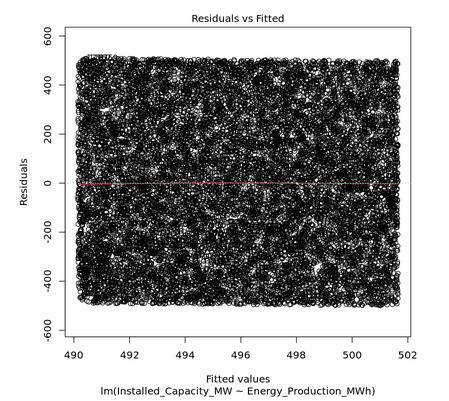
\includegraphics[width=1\linewidth]{lab4/obraz4.png}
    \caption{Lasso}
    \label{fig:enter-label}
\end{figure}

Wykonujemy walidację krzyżową i liczymy estymatę MSE:

\begin{Rcode}
cv_out <- cv.glmnet(X[train,], y[train], alpha = 1)
plot(cv_out)
cv_out$lambda.min
pred_lasso <- predict(fit_lasso, s = cv_out$lambda.min, newx = X[test,])
mean((pred_lasso - y[test])^2)
\end{Rcode}

\begin{figure}[H]
    \centering
    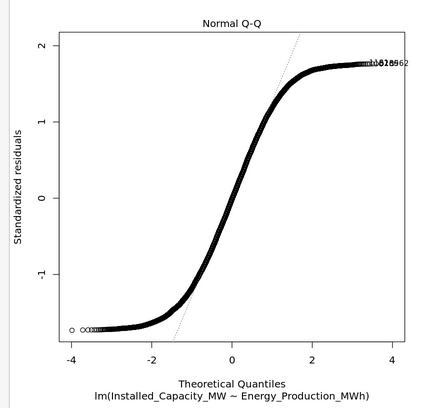
\includegraphics[width=1\linewidth]{lab4/obraz5.png}
    \caption{MSE a wartość $\lambda$ dla metody LASSO.}
    \label{fig:enter-label}
\end{figure}

Otrzymaliśmy MSE na poziomie \textbf{83114.31} - wynik trochę słabszy niż przy poprzednich metodach.

Sprawdźmy jeszcze wyniki dla optymalnej wartości parametru $\lambda$.

\begin{figure}[H]
    \centering
    \includegraphics[width=1\linewidth]{lab4/obraz5_5.png}
    \caption{MSE a wartość $\lambda$ dla metody LASSO o optymalnej wartości $\lambda$.}
    \label{fig:enter-label}
\end{figure}

Dla optymalnej wartości $\lambda \approx 6{,}3$ otrzymaliśmy wartość MSE 80114.

\subsection{Modele nieliniowe}

\subsubsection{Regresja wielomianowa}
Wykonajmy regresję wielomianową 4 stopnia dla \textbf{Air\_Pollution\_Reduction\_Index} na podstawie \textbf{Energy\_Production\_MWh}:

\begin{Rcode}
fit_poly <- lm(Air_Pollution_Reduction_Index ~ poly(Energy_Production_MWh, 4), data = energy_data)
\end{Rcode}

\begin{figure}[H]
    \centering
    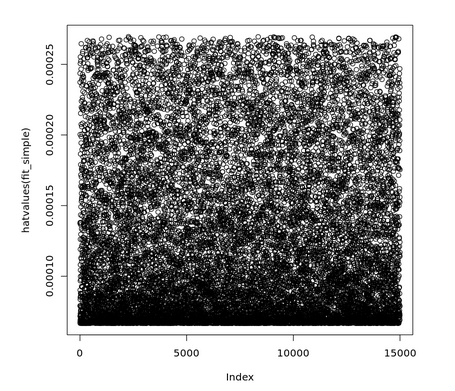
\includegraphics[width=1\linewidth]{lab4/obraz6.png}
    \caption{Wyniki regresji}
    \label{fig:enter-label}
\end{figure}

Z użyciem standardowej bazy wielomianów:
\begin{Rcode}
fit_poly_raw <- lm(Air_Pollution_Reduction_Index ~ poly(Energy_Production_MWh, 4, raw = TRUE), data = energy_data)
summary(fit_poly_raw)
\end{Rcode}

\begin{figure}[H]
    \centering
    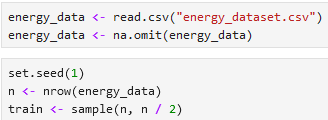
\includegraphics[width=1\linewidth]{lab4/obraz7.png}
    \caption{Wyniki regresji przy użyciu standardowej bazy wielomianów.}
    \label{fig:enter-label}
\end{figure}

Krzywa dopasowania:

\begin{figure}[H]
    \centering
    \includegraphics[width=1\linewidth]{lab4/obraz7_1.png}
    \caption{Krzywa dopasowania}
    \label{fig:enter-label}
\end{figure}

\subsubsection{Regresja logistyczna wielomianowa}
Podzielmy wartości w kolumnie Air\_Pollution\_Reduction\_Index na \textbf{High} i \textbf{Low}:

\begin{Rcode}
threshold <- 40
fit_log_poly <- glm(I(Air_Pollution_Reduction_Index > threshold) ~ poly(Energy_Production_MWh, 4), data = Wage, family = binomial)
\end{Rcode}

Spóbujmy wykonać predykcję:

\begin{Rcode}
pred_log_poly <- predict(fit_log_poly, list(Energy_Production_MWh = production_grid), se.fit = TRUE)
pred_probs <- plogis(pred_log_poly$fit)
se_bands_logit <- cbind(pred_log_poly$fit + 2 * pred_log_poly$se.fit,
                        pred_log_poly$fit - 2 * pred_log_poly$se.fit)
se_bands <- plogis(se_bands_logit)
plot(energy_data$Energy_Production_MWh, I(energy_data$Energy_Production_MWh > 40), xlim = production_lims, ylim = c(0, 1), 
     col = "darkgrey", cex = 0.5, ylab = "P(Air_Pollution_Reduction_Index > 40 | Energy_Production_MWh)")
lines(production_grid, pred_probs, col = "red", lwd = 2)
matlines(production_grid, se_bands, lty = "dashed", col = "red")
\end{Rcode}

\begin{figure}[H]
    \centering
    \includegraphics[width=1\linewidth]{lab4/obraz7_2.png}
    \caption{Dopasowanie wielomianu}
    \label{fig:enter-label}
\end{figure}

\subsubsection{Funkcje schodkowe}
Wykonajmy analogiczne dopasowanie funkcji schodkowej. Zacznijmy od podziału wartości na przedziały:

\begin{Rcode}
table(cut(energy_data$Air_Pollution_Reduction_Index, breaks = 4))
\end{Rcode}

Otrzymujemy w ten sposób przedziały:

\begin{figure}[H]
    \centering
    \includegraphics[width=1\linewidth]{lab4/obraz7_3.png}
    \caption{Enter Caption}
    \label{fig:enter-label}
\end{figure}

\begin{Rcode}
fit_step <- lm(Air_Pollution_Reduction_Index ~ cut(Energy_Production_MWh, 4), data = energy_data)
pred_step <- predict(fit_step, list(Energy_Production_MWh = production_grid), se.fit = TRUE)
se_bands <- cbind(pred_step$fit + 2 * pred_step$se.fit, 
                  pred_step$fit - 2 * pred_step$se.fit)
plot(energy_data$Energy_Production_MWh, energy_data$Air_Pollution_Reduction_Index, col = "darkgrey", cex = 0.5, xlim = production_lims)
lines(production_grid, pred_step$fit, col = "red", lwd = 2)
matlines(production_grid, se_bands, col = "red", lty = "dashed")
\end{Rcode}

\begin{figure}[H]
    \centering
    \includegraphics[width=1\linewidth]{lab4/obraz7_4.png}
    \caption{Dopasowanie schodkowe}
    \label{fig:enter-label}
\end{figure}

\subsection{Funkcje sklejane}
Użyjmy teraz funkcji sklejanych:

\begin{Rcode}
fit_bs_knots <- lm(Air_Pollution_Reduction_Index ~ bs(Energy_Production_MWh, knots = c(25, 40, 60)), data = energy_data)
pred_bs_knots <- predict(fit_bs_knots, list(Energy_Production_MWh = production_grid), se.fit = TRUE)
plot(energy_data$Energy_Production_MWh, energy_data$Air_Pollution_Reduction_Index, cex = 0.5, col = "darkgrey")
lines(production_grid, pred_bs_knots$fit, col = "red", lwd = 2)
lines(production_grid, pred_bs_knots$fit + 2 * pred_bs_knots$se.fit, col = "red",
      lty = "dashed")
lines(production_grid, pred_bs_knots$fit - 2 * pred_bs_knots$se.fit, col = "red",
      lty = "dashed")
abline(v = c(25, 40, 60), lty = "dotted")
\end{Rcode}

Zwiększenie stopnia wielomianu zwiększa dokładność przybliżenia.

\begin{figure}[H]
    \centering
    \includegraphics[width=1\linewidth]{lab4/obraz7_5.png}
    \caption{Dopasowanie funkcjami sklejanymi}
    \label{fig:enter-label}
\end{figure}

\subsubsection{Naturalne funkcje sklejane}
Użyjmy naturalnych wielomianów sklejanych:

\begin{Rcode}
fit_ns <- lm(Air_Pollution_Reduction_Index ~ ns(Energy_Production_MWh, df = 4), data = energy_data)
pred_ns <- predict(fit_ns, list(Energy_Production_MWh = production_grid), se.fit = TRUE)
plot(energy_data$Energy_Production_MWh, energy_data$Air_Pollution_Reduction_Index, cex = 0.5, col = "darkgrey")
lines(production_grid, pred_ns$fit, col = "red", lwd = 2)
lines(production_grid, pred_ns$fit + 2 * pred_ns$se.fit, col = "red",
      lty = "dashed")
lines(production_grid, pred_ns$fit - 2 * pred_ns$se.fit, col = "red",
      lty = "dashed")
abline(v = attr(ns(energy_data$Energy_Production_MWh, df = 4), "knots"), lty = "dotted")
\end{Rcode}

\begin{figure}[H]
    \centering
    \includegraphics[width=1\linewidth]{lab4/obraz7_6.png}
    \caption{Naturalne funkcje sklejane}
    \label{fig:enter-label}
\end{figure}

\subsubsection{Wygładzające funkcje sklejane}
Użyjmy wygładzjących funkcji sklejanych. Optymalny stopień wielomianu wyliczymy automatycznie przy pomocy walidacji krzyżowej:

\begin{Rcode}
fit_smooth_cv <- smooth.spline(energy_data$Air_Pollution_Reduction_Index, energy_data$Energy_Production_MWh, cv = TRUE)
plot(energy_data$Air_Pollution_Reduction_Index, energy_data$Energy_Production_MWh, cex = 0.5, col = "darkgrey")
lines(fit_smooth_cv, col = "red", lwd = 2)
\end{Rcode}

\begin{figure}[H]
    \centering
    \includegraphics[width=1\linewidth]{lab4/obraz7_7.png}
    \caption{Enter Caption}
    \label{fig:enter-label}
\end{figure}

\subsection{Uogólnione modele addytywne (GAMs)}
Teraz spróbujmy użyć modelu \textbf{GAM}, który można uczyć za pomocą metody najmniejszych kwadratów.

\begin{Rcode}
fit_gam_bf <- gam(Air_Pollution_Reduction_Index ~ s(Installed_Capacity_MW, df = 4) + s(Energy_Production_MWh, df = 5) + Energy_Consumption_MWh, data = energy_data)
summary(fit_gam_bf)

par(mfrow = c(1, 3))
plot(fit_gam_bf, col = "red", se = TRUE)
\end{Rcode}

Otrzymujemy takie dopasowania:
\begin{figure}[H]
    \centering
    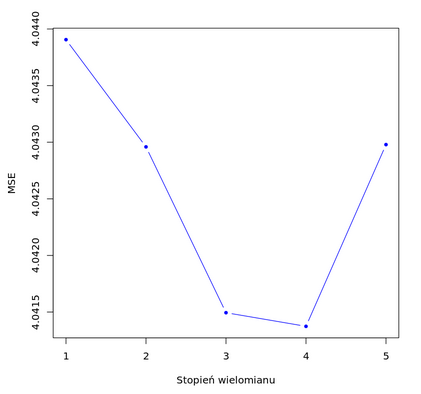
\includegraphics[width=1\linewidth]{lab4/obraz8.png}
    \caption{Różne dopasaowania wielomianów}
    \label{fig:enter-label}
\end{figure}

\subsection{GAM w GLM}
Przygotujmy regresję logistyczną wykorzystującą GAM:

\begin{Rcode}
fit_gam_1 <- gam(Air_Pollution_Reduction_Index ~ s(Installed_Capacity_MW, df = 5) + Energy_Production_MWh, data = energy_data)
fit_gam_2 <- gam(Air_Pollution_Reduction_Index ~ Energy_Storage_Capacity_MWh + s(Installed_Capacity_MW, df = 5) + Energy_Production_MWh, data = energy_data)
anova(fit_gam_1, fit_gam_2, fit_gam_bf, test = "F")
\end{Rcode}

Analiza odchyleń:

\begin{figure}[H]
    \centering
    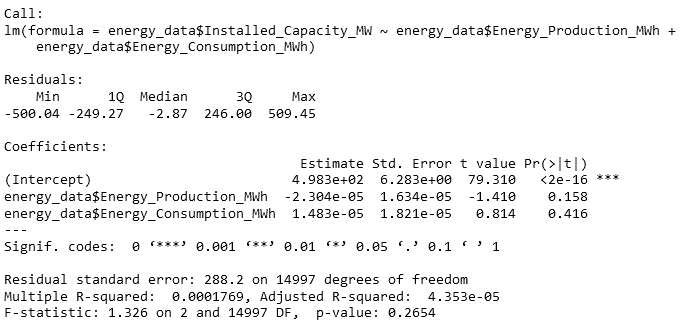
\includegraphics[width=1\linewidth]{lab4/obraz9.png}
    \caption{Analiza odchyleń}
    \label{fig:enter-label}
\end{figure}

Dopasowania:

\begin{figure}[H]
    \centering
    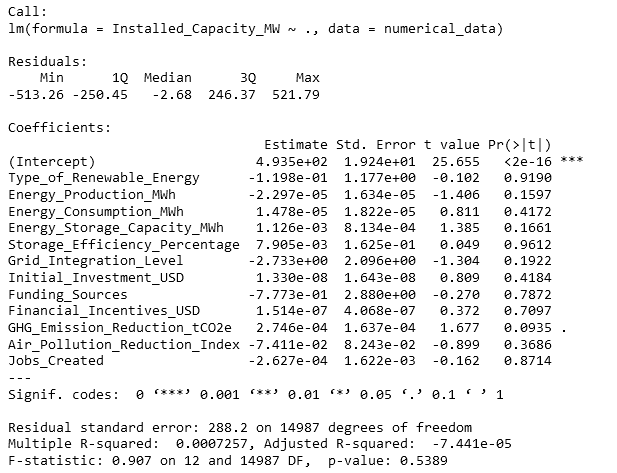
\includegraphics[width=1\linewidth]{lab4/obraz10.png}
    \caption{Enter Caption}
    \label{fig:enter-label}
\end{figure}
